% Options for packages loaded elsewhere
\PassOptionsToPackage{unicode}{hyperref}
\PassOptionsToPackage{hyphens}{url}
%
\documentclass[
  12pt,
]{article}
\usepackage{amsmath,amssymb}
\usepackage{iftex}
\ifPDFTeX
  \usepackage[T1]{fontenc}
  \usepackage[utf8]{inputenc}
  \usepackage{textcomp} % provide euro and other symbols
\else % if luatex or xetex
  \usepackage{unicode-math} % this also loads fontspec
  \defaultfontfeatures{Scale=MatchLowercase}
  \defaultfontfeatures[\rmfamily]{Ligatures=TeX,Scale=1}
\fi
\usepackage{lmodern}
\ifPDFTeX\else
  % xetex/luatex font selection
\fi
% Use upquote if available, for straight quotes in verbatim environments
\IfFileExists{upquote.sty}{\usepackage{upquote}}{}
\IfFileExists{microtype.sty}{% use microtype if available
  \usepackage[]{microtype}
  \UseMicrotypeSet[protrusion]{basicmath} % disable protrusion for tt fonts
}{}
\makeatletter
\@ifundefined{KOMAClassName}{% if non-KOMA class
  \IfFileExists{parskip.sty}{%
    \usepackage{parskip}
  }{% else
    \setlength{\parindent}{0pt}
    \setlength{\parskip}{6pt plus 2pt minus 1pt}}
}{% if KOMA class
  \KOMAoptions{parskip=half}}
\makeatother
\usepackage{xcolor}
\usepackage[margin=1in]{geometry}
\usepackage{graphicx}
\makeatletter
\def\maxwidth{\ifdim\Gin@nat@width>\linewidth\linewidth\else\Gin@nat@width\fi}
\def\maxheight{\ifdim\Gin@nat@height>\textheight\textheight\else\Gin@nat@height\fi}
\makeatother
% Scale images if necessary, so that they will not overflow the page
% margins by default, and it is still possible to overwrite the defaults
% using explicit options in \includegraphics[width, height, ...]{}
\setkeys{Gin}{width=\maxwidth,height=\maxheight,keepaspectratio}
% Set default figure placement to htbp
\makeatletter
\def\fps@figure{htbp}
\makeatother
\setlength{\emergencystretch}{3em} % prevent overfull lines
\providecommand{\tightlist}{%
  \setlength{\itemsep}{0pt}\setlength{\parskip}{0pt}}
\setcounter{secnumdepth}{5}
\usepackage{float}
\usepackage{sectsty}
\usepackage{paralist}
\usepackage{setspace}
\usepackage{fancyhdr}
\usepackage{lastpage}
\usepackage{dcolumn}
\usepackage{natbib}\bibliographystyle{agsm}
\usepackage[nottoc, numbib]{tocbibind}
\ifLuaTeX
  \usepackage{selnolig}  % disable illegal ligatures
\fi
\IfFileExists{bookmark.sty}{\usepackage{bookmark}}{\usepackage{hyperref}}
\IfFileExists{xurl.sty}{\usepackage{xurl}}{} % add URL line breaks if available
\urlstyle{same}
\hypersetup{
  pdftitle={Masters Thesis: Coded in R},
  pdfauthor={Robert J. Dellinger},
  hidelinks,
  pdfcreator={LaTeX via pandoc}}

\title{Masters Thesis: Coded in R}
\author{\href{https://robdellinger.com}{Robert J. Dellinger}}
\date{2024}

\begin{document}
\maketitle

\newpage
\pagestyle{empty}

\allsectionsfont{\centering}
\subsectionfont{\raggedright}
\subsubsectionfont{\raggedright}

\begin{centering}

\vspace{1 in}
{\bf CALIFORNIA STATE UNIVERSITY, NORTHRIDGE}

\vspace{0.1 in}
{Department of Biology}
\vspace{0.2 in}




\includegraphics[width=0.3\linewidth]{Images/university_logo} 


\vspace{0.1 in}

\doublespacing
{\bf Facing Physiological Plasticity: Investigating the Interactive Effects of pH and Temperature Variation on the Metabolic Demand of an Intertidal Gastropod \emph{Tegula funebralis} Amidst a Fluctuating Tidal Environment \\}

\vspace{0.3 in}

Thesis submitted in partial fulfillment of the requirements\\
For the degree of Master of Science in Biology \\

\vspace{0.4 in}
\singlespacing
By

\vspace{0.1 in}
{Robert J. Dellinger}

\vspace{2 in}
May 2024

\end{centering}
\doublespacing

\newpage
\pagestyle{plain}
\pagenumbering{roman}

\section*{}

\vfill

\begin{center}
Copyright by Robert J. Dellinger
\end{center}

\newpage

The thesis of Robert J. Dellinger is approved:

\vspace{1.5in}

\underline{\hspace{2.5in}}\hspace{0.5in} \underline{\hspace{2in}}

Dr.~Peter J. Edmunds \hspace{1.65in} Date:

\vspace{0.5in}

\underline{\hspace{2.5in}}\hspace{0.5in} \underline{\hspace{2in}}

Dr.~Kerry J. Nickols \hspace{1.75in} Date:

\vspace{0.5in}

\underline{\hspace{2.5in}}\hspace{0.5in} \underline{\hspace{2in}}

Dr.~Nyssa J. Silbiger, Chair \hspace{1.3in} Date:

\vfill

\begin{center}
California State University, Northridge
\end{center}

\newpage

\vspace*{\fill}

\begin{center}

\begin{minipage}{0.8\textwidth}
\begin{quote}

``Against this cosmic background the lifetime of a particular \\
  plant or animal appears, not as a drama complete in itself, \\
  but only as a brief interlude in a panorama of endless change.'' \\

— Rachel Carson, \textit{Undersea} (1937)
\end{quote}
\end{minipage}

\vspace*{\fill}

\begin{minipage}{0.8\textwidth}
\begin{quote}
``For nothing is fixed, forever, forever, forever, \\
  it is not fixed; \\
  the earth is always shifting, \\
  the light is always changing, \\
  the sea does not cease to grind down rock.\\
  Generations do not cease to be born,\\ 
  and we are responsible to them \\
  because we are the only witnesses they have. \\
 
  The sea rises, the light fails, \\
  lovers cling to each other, \\
  and children cling to us. \\
  The moment we cease to hold each other, \\
  the moment we break faith with one another, \\
  the sea engulfs us and the light goes out.'' \\


— James Baldwin, \textit{Nothing Personal} (1964)
\end{quote}
\end{minipage}

\vspace*{\fill}

\end{center}

\newpage

\section*{Acknowledgements}

~~~~~ First and foremost, I would like to express my gratitude to our
ocean for the generosity it bestows upon us daily and for the awe it
instilled in me as a young child---a wonder that has grown into a
lifelong dream and pursuit. I am deeply grateful to Dr.~Nyssa J.
Silbiger, my advisor, for her unwavering support, encouragement,
inspirational attitude, and collaboration on this project. Thank you for
believing in me, urging me to become the person I need to be, equipping
me with the knowledge, tools, and skills needed to achieve this, and for
ignoring the lies we often tell ourselves about ourselves. To my thesis
committee, Dr.~Peter J. Edmunds and Dr.~Kerry J. Nickols, thank you for
your invaluable guidance and advice throughout this process. Thank you
to my mentors, Dr.~Aradhna Tripati, Dr.~Rachel Bay, Dr.~Tessa Hill, and
Dr.~Melanie Okoro, who have acted as academic mothers, paving the way
and uplifting me throughout my academic trajectory. I would also like to
extend my gratitude to the Silbiger and Nichols Lab team, including D.M.
Barnas, J.R. Kerlin, C. Fajardo, and H. Merges. In particular, I want to
give a special thank you to J.B. Fields and T. Smith for their
monumental support and dedication in ensuring that everything ran
smoothly inside and outside of the lab; they were always there as
friends to call on and played pivotal roles in ensuring the success of
my degree. Without all of you, none of this would have been possible.
Throughout endless sleepless nights and days of struggle, thank you for
lifting as you climbed. A special thank you to Ana and the rest of the
custodial staff, whose skills are the cornerstone of the entire
institution, and whose presence makes the halls of academia feel more
like home as they sweep through the halls, serenaded by the rhythm of
bachata. This research couldn't have been possible without the financial
support from the National Science Foundation Graduate Research
Fellowship Program, UCLA Center for Diverse Leadership in Science Early
Career Fellowship, UC Davis Sustainable Oceans Scholars Program, and the
National Science Foundation CAREER grant OCE-2044837 awarded to
Dr.~Nyssa Silbiger, the material in this study based upon work supported
by the U.S. National Science Foundation, the CSUN Department of Biology,
and research activities that were conducted under scientific collecting
permits issued by the California Department of Fish and Wildlife (ID:
S-220520002-22054-001).

~~~~~ I extend my heartfelt gratitude to my family, Robert K. Dellinger
and Ana. C. Dellinger, for instilling in me the belief that education is
the most powerful tool. They have made me feel capable of achieving
anything I set my mind to and have unwaveringly supported my dreams,
regardless of their nature. To my father, thank you for raising me with
the understanding that everything we create must be done with love; love
is the secret ingredient. To my mother, I am forever thank you for
sacrificing your own dreams and for persevering through the challenges
of the ingratitude of the nation in which you settled, all to ensure
that I could pursue my own dreams and aspirations.Thank you to all of
those who have parented me and the push of the universe for laughing at
me. Thank you to my chosen family, including my partner and friends, who
immersed me in a queerness that dominant systems cannot understand, who
illuminated alternative paths from the outdated paradigms we are
entangled in, and who remember to swim despite everything. Their love
and resilience have nurtured me and imbued me with the buoyancy and
fortitude to demand better from the world around me. Thank you for your
willingness to churn the waters up, for being holders of wisdom and
knowledge, and for showing me that the facts of nature often falsify the
prevailing theories. I would not be here today without their love and
support.

~~~~~ Being a part of the CSUN and the Los Angeles community the past
three years has been some of the most formative and fulfilling
experiences of my life and for my career moving forward. Studying
climate change in an era marked by rapid ecological change and numerous
interconnected crises, encompassing racial capitalism and the climate
emergency, particularly during a time in which society stands at a
pivotal crossroads for humanity's future can feel rather dismal. Yet the
support and knowledge I've received from my community and mentors as
well as the collective imagination of the communities I am a part of has
instilled within me an unbridled sense of optimism. That amid these
challenges, we possess all of the solutions to the crises we face, and
that within our collectivities, there are reservoirs of hope for the
future - a future where our individual lives matter not less, but more,
as they form the pixels shaping a panorama of endless change.

\centering
\raggedright
\newpage
\tableofcontents

\newpage
\listoftables

\newpage
\listoffigures
\newpage

\pagenumbering{arabic}

\section*{Abstract}

Ocean acidification (OA) is occurring across a backdrop of concurrent
environmental changes that may in turn influence species' responses to
OA. Temperature affects many fundamental biological processes and
governs key reactions in the seawater carbonate system. It therefore has
the potential to offset or exacerbate the effects of OA. While initial
studies have examined the combined impacts of warming and OA for a
narrow range of climate change scenarios, our mechanistic understanding
of the interactive effects of temperature and OA remains limited. Here,
we use the black turban snail, Tegula funebralis, as a model species to
test how OA affects the respiration rate of a herbivorous invertebrate
across a wide range of temperatures encompassing their thermal optimum.
Snails were exposed in the laboratory to a factorial combination of low
and high pCO2 (400 and 1200 µatm CO2) and temperatures (12, 14, 16, 18,
20, 22, 24, 26°C) for two weeks. Results indicate that the effects of OA
on respiration rate are highly dependent on temperature. Although high
CO2 significantly increased respiration rate at 20°C, this effect
gradually lessened with successive warming to 20°C, illustrating how
moderate warming can mediate the effects of OA through temperature's
effects on both physiology and seawater geochemistry. Together, these
results highlight the importance of considering the physiological and
geochemical interactions between temperature and carbonate chemistry
when interpreting species' vulnerability to OA.

\newpage

\hypertarget{introduction}{%
\section{Introduction}\label{introduction}}

~~~~~ Organisms and environments are entwined, as the relationship
between organisms and the environments they are embedded within, is in
constant flux through inextricable links and flows of energy. The
relationship between organisms and environments varies through both
space and time and is influenced by a mosaic of dynamic biotic and
abiotic drivers \cite{connell1977mechanisms, menge1987community}.
Organisms are active participants in constructing their environment,
from altering seawater biogeochemistry through physiological processes
to organisms constructing biogenic structures; plenty of studies
demonstrate that organisms influence their environment
\cite{lewontin1983organism,estes1974sea}. Organisms and ecosystems,
while playing an essential role in structuring the physical and
biological environment, are simultaneously governed by the ability to
perform and function under a myriad of complex interactions, as each act
to influence one another non- contemporaneously and contemporaneously
through direct and indirect feedback loops
\cite{levin1974disturbance,paine1980food}. Organisms must
physiologically cope with the conditions of the environment they are
situated within, which inevitably influences community structure and
populations \cite{bozinovic2015physiological}. Further, the biogenic
structures created by organisms are highly dependent upon the
environmental regime the organism develops in, living beyond the life of
the organism itself; organisms are thus simultaneously creators and
products of the environment. In a geological epoch of rapid ecological
change, it is increasingly imperative to understand how and the extent
to which organisms can respond and perform to abiotic drivers and how
the legacy of the structures (e.g., shells, reefs) that organisms create
may influence other species indirectly. Understanding physiological
responses, interactions, and constraints of marine organisms to
anthropogenic climate change is perhaps the sine qua non for
understanding the changes between marine organisms and the ecosystems
they construct. This research intends to inform how the changing oceanic
environment may affect organismal physiology by teasing apart the
relationship between environmental drivers and physiological
performance. This research also intends to elucidate how changes within
physiological processes in one organism may have indirect effects on
other species long after the organism persists. In this regard, the fate
of organisms is intertwined as the abundance and growth of one species
codetermines the other, illustrating that organisms are directly or
indirectly the subjects and objects of ecological change
\cite{lewontin1983organism}.

\hypertarget{organisms-as-the-subjects-of-ecological-change}{%
\section{Organisms as the Subjects of Ecological
Change}\label{organisms-as-the-subjects-of-ecological-change}}

~~~~~Environments are governed by natural spatiotemporal variation of
abiotic and biotic drivers that, in turn, influence the structure and
processes of communities, drive ecological change, and create a mosaic
of microhabitats
\cite{connell1961influence, stenseth2002ecological, kroeker2017embracing}.
For example, within marine ecosystems, the combination of oceanographic
processes and local coastal geography may create an array of patterns
and variability in abiotic drivers such as temperature, flow, pH,
dissolved oxygen, etc., that may impact the structure and processes of
ecological communities on distances ranging from microscale to
macroscale \cite{deser2010sea, hofmann2010living}. Such heterogeneous
patterns are naturally occurring and create complex gradients that shape
ecological communities and influence physiological processes within
individual organisms \cite{helmuth2006mosaic}. However, due to the
connotation of stress as a negative response and the ability for
organisms to adapt and evolve to changing conditions over time, the term
driver has been utilized to describe an environmental parameter that
influences organisms and environments across a spectrum ranging from
enhancing, optimal, or stressful conditions
\cite{cote2016interactions, boyd2012understanding}. Many organisms have
evolved to withstand complex and variable environmental gradients
through physiological mechanisms such as phenotypic plasticity and
acclimatization \cite{hofmann2010living, tomanek2002heat}. According to
the metabolic theory of ecology, environmental gradients and changes in
abiotic factors may result in physiological trade-offs due to the
alterations within the energetic partitioning of an organism's
metabolism \cite{portner2008physiology, brown2004toward}. The
physiological processes of metabolism are the total sum of biological
and chemical processes in converting energetic resources and materials
into biomass and activity \cite{brown2004toward}. Comparing
physiological responses to gradients of abiotic drivers may allow us to
quantify and compare the tolerance limits of organisms
\cite{somero2002thermal, silbiger2019comparative}. The role of biotic
and abiotic drivers in influencing metabolic processes has been of
primary interest to the field of ecology as changes in metabolism
directly affect the survival, behavior, and energy requirements of
organisms, thereby impacting fitness and ecosystem function
\cite{carey2016sea}.

~~~~~ Temperature and pH are important for determining physiological
processes and metabolic rates for marine organisms and thereby play a
large role in affecting the functioning and physiology of ecosystems
\cite{woodwell1970effects}. Temperature is the key driver in determining
physiological rates of organisms as the kinetic energy of biochemical
reactions is temperature dependent
\cite{levins1968evolution, somero2002thermal, portner2012integrating}.
Biological processes such as organismal and ecological interactions are
also strongly influenced by temperature \cite{hochachka2002biochemical}.
The relationship between temperature and body-size exemplifies this as
organisms develop faster yet decrease in size under elevated
temperatures \cite{elahi2020historical}. Metabolic rates are strongly
influenced by an organism's body size and temperature and are subject to
change due to changes in abiotic drivers and the natural variability of
drivers \cite{brown2004toward, o2007temperature}. Further, organisms
adapt to local temperatures to match optimal conditions for
physiological processes and acclimatize to a range around these values
\cite{sinclair2016can}. Any range too far beyond the ability of an
organism to acclimatize influences survival, fitness, and population
densities \cite{hochachka2002biochemical}. Studies have shown the
influence of sea surface temperature on metabolic processes such as
growth, feeding, reproduction, and influencing the range of species
distributions
\cite{kordas2011community, sanford2002feeding, pinsky2013marine}.
However, it is essential to note that temperature is not the only driver
of biological processes and temperature has interactive effects with
other abiotic drivers \cite{darling2008quantifying}. pH is also an
important abiotic driver that impacts the physiological performance of
marine organisms and influences the biogenic structures that organisms
create \cite{hofmann2010living}. pH plays a vital role in metabolic
processes due to its effect on biochemical pathways and internal
acid-base balance \cite{gaylord2015ocean}. For example, low pH is often
associated with elevated metabolic rates due to the increase in
energetic costs in creating calcified structures such as the formation
of shells in mollusks or the skeletons of corals and echinoderms
\cite{doney2009ocean, spalding2017energetic}. Due to differences in the
energetic costs associated with calcification, there are significant
differences in the ability to control acid-base regulation between
species \cite{doney2009ocean}. Consequently, changes in physicochemical
parameters of the environment affect species differently, impact the
interaction between species and, in turn, affect the structures of
ecological communities; therefore, studying how differences between
abiotic drivers affect organismal physiology will have ecosystem-level
implications \cite{tomanek2002physiological, barclay2019variation}.

\hypertarget{organismal-physiology-in-a-changing-environment}{%
\section{ORGANISMAL PHYSIOLOGY IN A CHANGING
ENVIRONMENT}\label{organismal-physiology-in-a-changing-environment}}

~~~~~ As the atmospheric carbon dioxide (CO2) concentration continues to
surpass the limits of the earth system, marine organisms will be forced
to endure profound transformations of the envrionment, from shifts in
temperature to altered geochemistry (richardson2023earth,
portner2008physiology\}. Ocean warming (OW) and ocean acidification (OA)
represent two of the most significant changes occurring in marine
ecosystems across the globe, both driven by the unremitted rise of
anthropogenic-induced carbon dioxide emissions. OW and OA are not
isolated phenomena; they share a common origin, and in a rapidly
changing world, their combined impacts on organismal physiology
necessitate special attention as multiple drivers of change may act
interactively \cite{cote2016interactions}. Since the beginning of the
20th century, the global mean sea surface temperature (SST) has
increased by 0.88 {[}0.68--1.01{]} °C, and is further projected to warm
by 2.89°C {[}2.01--4.07°C{]} at the end of the century, which surpasses
the thermal tolerance limits of many marine species (following the
representative concentration pathway 8.5 emission scenario)
\cite{kikstra2022ipcc, fox2021ocean, bay2017genomic, somero2010physiology}.
Concurrently, the ocean has absorbed \textasciitilde30\% of
anthropogenic CO2 \cite{feely2004impact}, altering the carbonate
chemistry of seawater through a decrease in the concentration of
carbonate ions \(\mathrm{CO_3^{2-}}\) and a decline in seawater pH
\cite{feely2004impact}. Mean surface ocean pH values have declined by
0.1 units since the pre-industrial era, with a further projected
diminution of 0.1 - 0.4 units by the end of the century
\cite{change2014impacts, orr2005anthropogenic}, posing a unique threat
to calcifying marine organisms. Consequently, the impacts of OW and OA
will not be consistent across geographic regions, leading to
differential effects that will modify already variable spatial and
temporal environments. Building a mechanistic understanding of how the
combined impacts of ocean warming and acidification affect marine
organisms is integral for reliable projections of how climate change may
continue to affect marine organisms.

~~~~~ Coastal marine organisms frequently encounter a wide range of
temperatures and experience fluctuations in biogeochemistry, resulting
from temporal variations, such as tidal and seasonal cycles. The rocky
intertidal system is one such system that is known for its variable
conditions on both temporal and spatial scales, making them a model
ecosystem for understanding how organisms interact and respond to change
\cite{connell1961influence, paine1969pisaster, kwiatkowski2016nighttime, jellison2022low}.
Organisms within the rocky intertidal zone must contend with alternating
periods of immersion and emersion of tidal fluctuations, which commonly
lead to large variations in temperature, oxygen availability, and pH,
\cite{denny2001physical; helmuth2002climate}. Of these naturally
occurring changes, thermal variability within the intertidal zone is
believed to be a dominant driver in structuring the vertical and
latitudinal distribution patterns by limiting upper zonation through
abiotic stress and lower zonation through biotic influence
\cite{helmuth2006mosaic; somero2002thermal, somero2010physiology, connell1961influence}.
Daily temperature fluctuations are drastic enough to elevate the body
temperatures of marine organisms by more than 20°C during a tidal
emersion event \cite{Helmuth, 1999}. Furthermore, changes in pH within
tidepools may exceed 1 unit when nighttime respiration rates exceed
photosynthetic rates \cite{jellison2016ocean, kwiatkowski2016nighttime}.
Such highly variable abiotic changes are naturally occurring and create
complex gradients that shape ecological communities and influence
physiological processes within individual organisms
\cite{helmuth2006mosaic}. Given that organisms within the intertidal
zone simultaneously face drastic fluctuations from abiotic drivers, and
experience conditions far beyond what is expected in the future,
understanding organismal performance in these ecosystems may provide a
window for looking toward the future.

~~~~~ The role of biotic and abiotic drivers in influencing metabolic
processes has been of primary interest to the field of ecology as
changes in metabolism directly affect the survival, behavior, and energy
requirements of organisms, thereby impacting organism and ecosystem
function \cite{Carey, Harianto, & Byrne, 2016}. Physiological processes
are heavily influenced by environmental factors, and many marine
organisms undergo biological responses to natural diel variability
present within environments \textbackslash cite\{hofmann2010living.
Temperature is the primary environmental driver regulating physiological
rates of ectothermic organisms, as kinetic energy of biochemical
reactions are temperature dependent
\cite{levins1968evolution, huey1979integrating, hochachka2002biochemical}.
Further, temperature is the key determinant in the regulating rates of
biological processes, ranging from metabolic rates
\cite{gillooly2001effects} to species-interactions
\cite{sanford1999regulation}, such as growth, feeding, reproduction, and
determining the range of species distributions
\textbackslash cite\{kordas2011community, sanford2002feeding,
pinsky2013marine. The physiological processes of metabolism are the
total sum of biological and chemical processes in converting energetic
resources and materials into biomass and activity
\cite{brown2004toward}. Changes in pH also play a vital role in
metabolic processes due to its effect on biochemical pathways and
internal acid-base balance \cite{gaylord2015ocean}. Specifically,
declines in seawater carbonate ions and pH attributed to OA are strongly
correlated to decreases in calcification and growth rates of many marine
organisms \cite{kroeker2013impacts}. Due to species-specific differences
in the energetic costs associated with calcification, there are
significant differences in the ability to control internal acid-base
regulation between species \cite{doney2009ocean}. Ultimately, changes in
the environment that lead to alterations in organismal energetic
requirements will scale up to affect the processes of ecological
communities; therefore, studying how multiple abiotic factors affect
organismal physiology has ecosystem-level implications
\cite{tomanek2002heat, barclay2019variation, kroeker2022ecological}.

\begin{figure}[htbp]
    \centering
    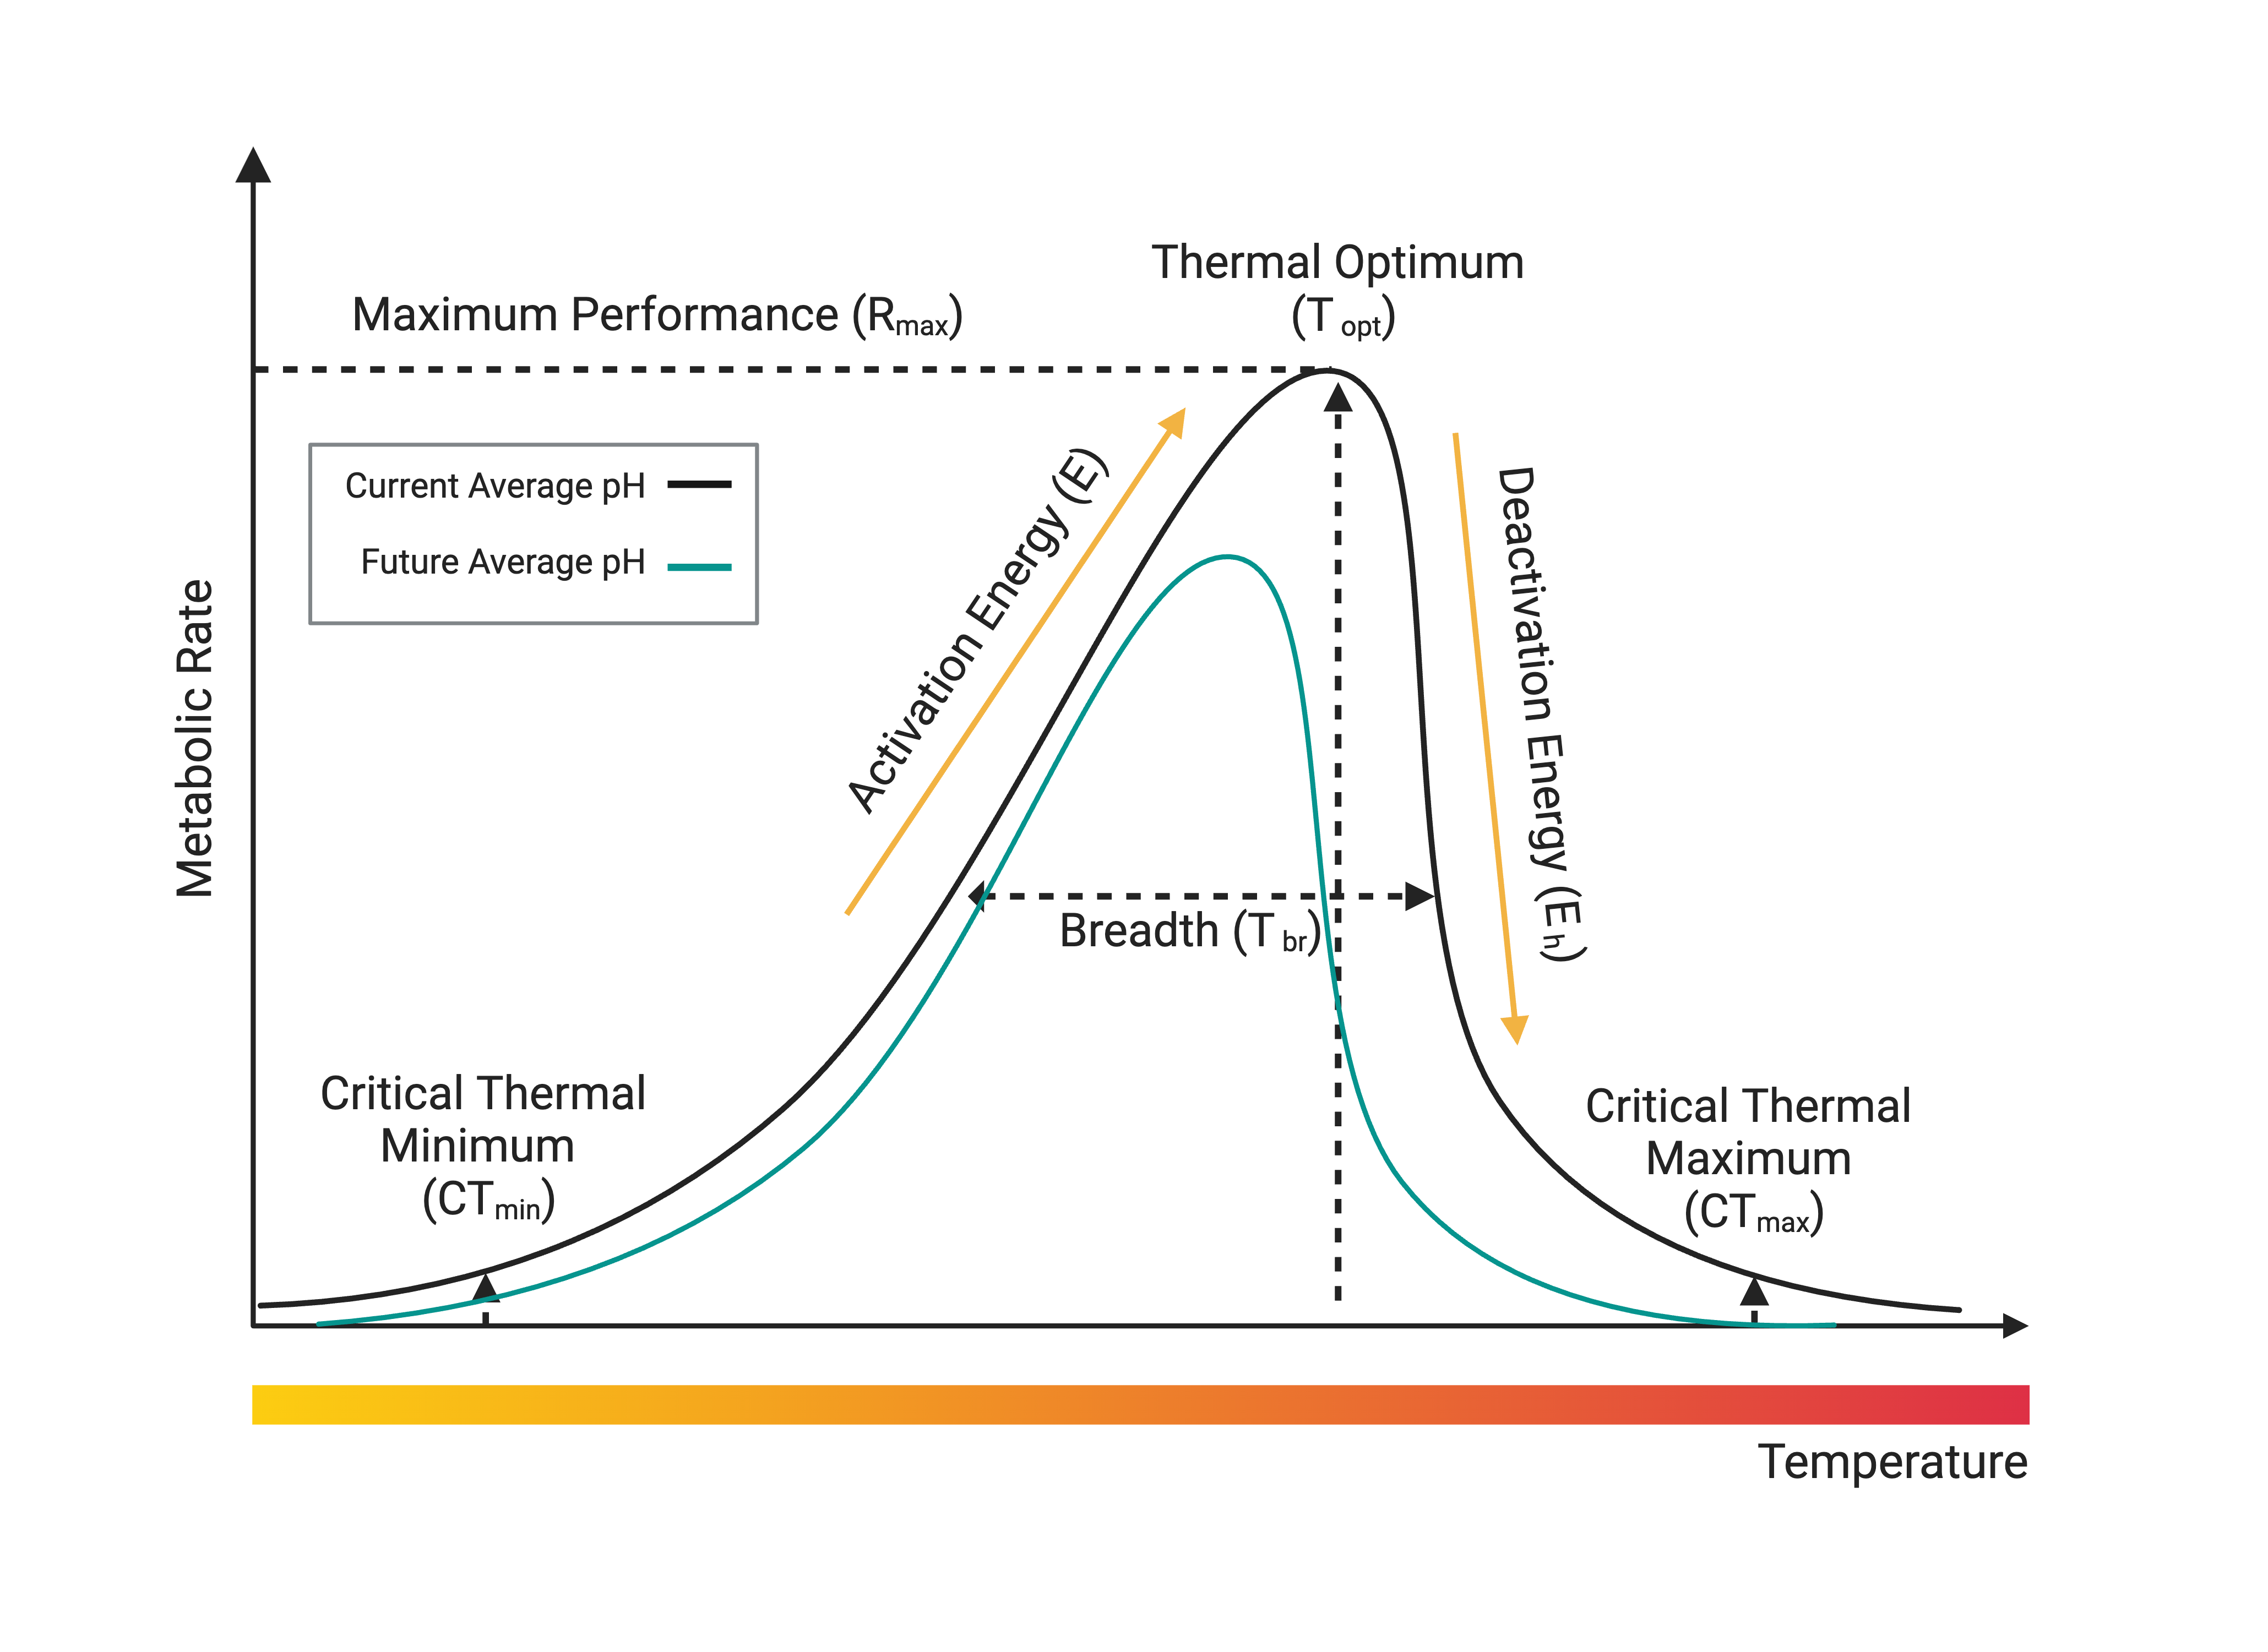
\includegraphics[width=1\textwidth]{Images/thermal_performance_curve_schematic.png}
    \caption{Thermal performance curve schematic illustrating the relationship between biological rates and temperature, including critical thermal maximum (CTMax), critical thermal minimum (CTMin), thermal optimum (Topt), activation energy (E), deactivation energy (Eh), and the thermal breadth of the curve (TBr). Hypothesized characteristics of a thermal performance curve exposed to ocean acidification, including reduced thermal optimum and reduced performance ay maximum physiological rate and breathe of the curve.}
    \label{fig:Thermal Performance Curve Schematic}
\end{figure}

~~~~~ The use of performance curves can help to quantify the
relationship between abiotic drivers and physiological rates to forecast
future effects \cite{kroeker2017embracing} and can allow for comparative
assessments across different biological rates and environmental
conditions (Figure 1.)
\cite{schulte2011thermal, silbiger2019comparative, silva2021local, padfield2021rtpc; becker2020nutrient}.
Further, thermal performance curves have been suggested to fill in the
gap of uncertainty between multiple stressors as they empirically
characterize the relationship between biological performance rates
across a wide range of temperatures
\cite{padfield2021rtpc, schulte2011thermal, silbiger2019comparative}.
Thermal performance curves are a univariate function that describes how
some measure of performance (e.g., metabolic rate) varies with
temperature. As temperature increases so do the biochemical and
physiological rates until they reach a species-specific optimal
temperature. Beyond the optimum rate, further increases in temperature
denature proteins, stunt growth, and cause reductions in performance and
survival \cite{somero2002thermal, portner2002climate}. Thermal
performance curves are typically left-skewed and hump-shaped and include
several metrics, including but not limited to a thermal optimum
(TOpt)---the temperature at the highest rate of performance---and a
critical thermal minimum (CTMin) and a thermal maximum (CTMax)--- the
upper and lower thermal limit that an organism can tolerate
\cite{schulte2011thermal, huey1979integrating, huey1989evolution}. These
tolerance thresholds and the range they encompass are governed by an
organism's ability to respond to sub-lethal and lethal conditions
through an organismal-level response and molecular-level responses such
as anaerobic metabolism and heat shock response
\cite{portner2017oxygen, somero2002thermal}. Further, exposure to
concurrent drivers of ecological change, like OA, are expected to
constrict an organism's performance curve and thermal limits, such as
decreasing the breadth of thermal performance
\cite{portner2008physiology, portner2010oxygen}. Comparing physiological
responses to gradients of abiotic drivers may allow us to quantify and
compare the tolerance limits of organisms
\cite{silbiger2019comparative}.

~~~~~ Specifically, we ask the question: how does exposure to decreased
pH influence thermal performance curves of respiration of an intertidal
gastropod, Tegula funebralis? We anticipate that the thermal optimum
(TOpt) for respiration rates will shift towards lower temperatures,
indicating a reduced ability to sustain optimal metabolic activity in
the face of ocean acidification. Additionally, we expect a decrease in
the thermal breadth of the curve (TBr), indicating a narrower range of
temperatures at which the gastropod can effectively maintain its
respiratory rates. In this study we\ldots(give an overview of your
experimental design to set up expectations on how you plan to answer
these questions)

\newpage

\hypertarget{methods}{%
\section{Methods}\label{methods}}

\vspace{0.5cm}

\hypertarget{mesocosm-design}{%
\subsection{(1) Mesocosm Design}\label{mesocosm-design}}

~~~~~The Silbiger Lab mesocosm system at California State University,
Northridge was used to emulate experimental conditions of a semi-diurnal
tidal fluctuation across a gradient of temperatures and blocked exposure
to either low or high pH. The facility operated as a closed-loop system,
wherein water from individual tanks was continuously recirculated back
into a central holding reservoir (sump). Unbuffered natural seawater was
collected from the Southern California Marine Institute (SCMI) in San
Pedro, CA and filtered through three mesh filters (20 \(\mu\)m, 5
\(\mu\)m, 1 \(\mu\)m) prior to being introduced into the sump of the
mesocosm system. Within the system, recirculating seawater underwent
further filtration through three 50 \(\mu\)m carbon bag filters, eight
mesh filters, a UV sterilizer (Comet Series 95 Watt Lamp), and a chiller
(Aqua Logic Delta Star, DS-4) which maintained water quality and chilled
seawater to ambient conditions. Weekly water replacements, accounting
for approximately 50\% of the total volume, were conducted to prevent
the accumulation of metabolic waste and to maintain stable carbonate
parameters within the system. The mesocosm system was equipped with 16
experimental tanks (53.9 cm (L) × 31.75 cm (W) × 34.29cm (H)) with
individual controls for temperature, light intensity, and water flow.
Each tank was outfitted with a submersible powerhead pump (Hydor Nano
Koralina 240 powerhead, 240 GPH), 200 W Heater (Hydor aquarium heater),
temperature probe (Neptune Systems, ±0.1 degree C), pH probe (Neptune
Systems, Lab Grade Double Junction, measures pH from 4.0 to 12.0 ±0.1),
three flow sensors (Apex, FS25 ¼'' fitting, flow rates from 3-12 GPH
(12-24 LP)), and a temperature logger (HOBO TidBit MX2203, ±0.2 degree
C). LED lights (Halo Basic M-110) in each tank followed a 12:12
day/night cycle, which mimicked the local light conditions using a
sunset and sunrise table.

~~~~~Each individual tank was programmed to experience tidal
fluctuations as well as temperature/pH controlled seawater conditions
for their respective treatments. Programmable solenoid valves (Apex
Neptune) were utilized to adjust the seawater flow rates to each tank,
ensuring that either inflow rates exceeded outflow drain rates
simulating a high tide condition or outflow drain rates exceeded inflow
rates to simulate a low tide condition. This emulation aimed to
replicate the semi-diurnal tidal characteristic of the Pacific Coast.
Within a 24-hour period, two high tide and two low tide fluctuations,
each lasting six hours, were generated by either opening or closing the
solenoids. Flow rates were meticulously maintained on a daily basis
using a graduated cylinder and timepiece to ensure a programmable inflow
of 10 L/h, constant total inflow of 10 L/hour, and a constant outflow
drain rate of 15 L/hour, thereby creating the desired tidal effect.
Precise control over temperature in each tank was achieved by employing
a programmable thermostat (Neptune Apex), which automatically activated
or deactivated heaters in response to temperature deviations from the
set range. Individual tank pH levels were regulated using a pH-stat
set-up through the direct bubbling and mixing of CO2 facilitated by a pH
logger and solenoid valves (Neptune system) attached to a CO2 tank
(PhosBan Reactor 150). Additionally, in each tank, a venturi connected
to an aquarium pump facilitated the mixing of ambient air to stabilize
the pH levels in the treatment tanks. After recirculation into the sump
system, the sweater was chilled to ambient condition and scrubbed of CO2
using a phosban reactor (Phosban 150 Reactor).

~~~~~Throughout the experiment, various water quality parameters were
regularly measured to monitor environmental conditions within the tanks.
pH, dissolved oxygen (DO), and temperature were assessed daily at
consistent times to ensure accurate readings and facilitate the
calibration of in-tank temperature probes for precise measurements. pH
and dissolved oxygen levels were measured daily, within each tank using
a Termo Specific ORION ISE instrument with a resolution of 0.1 mV and an
accuracy of ±0.2 mV or ±0.05\%. Simultaneously, temperature readings
were obtained using a Thermo Fisher Trace digital thermometer. The
temperature data also aided in calibrating the thermostat sensors within
each tank, which were adjusted once a day to maintain accurate
temperature control. pH on the total scale was calculated from mV and
temperature by using a multipoint calibration to a tris standard
solution from the Dickson Lab at Scripps Institution of Oceanography
following Dickson SOP 6a \cite{dickson2007guide}. Accuracy of the pH was
tested against a Tris buffer of known pH from the Dickson Lab at Scripps
Institution of Oceanography \cite{dickson2007guide}. The pH values for
the individual aquaria were calculated using the seacarb package in R,
accounting for temperature corrections specific to each tank
\cite{gattuso2015package}. I also measured total alkalinity (TA) from
water samples collected once every few days (3-4 days) from each
experimental tank and sump. All total alkalinity (TA) water samples were
collected and stored in 125 ml Nalgene containers. Prior to use, these
containers underwent thorough cleaning in a 10\% HCl bath for 24 hours,
followed by rinsing with deionized (DI) water. Additionally, during
sample collection, the containers were rinsed three times with sample
water to ensure a representative water quality sample. Collected samples
were analyzed within 24 hours of collection using a T-5 automatic
titrator (Mettler Toledo) following the best practices for ocean CO2
measurements \cite{dickson2007guide}. To verify accuracy, a certified
reference material (Reference Material for Oceanic CO2 Measurements, A.
Dickson, Scripps Institution of Oceanography) was run prior to each
total alkalinity measurement with an error no greater than 1.0\% off
from the certified value \cite{dickson2007guide}.

\hypertarget{insert-table.-summary-statistics-means-se-for-tank-parameters-at-each-of-the-three-timepoints.}{%
\subsubsection{INSERT TABLE. Summary statistics (means ± SE) for tank
parameters at each of the three
timepoints.}\label{insert-table.-summary-statistics-means-se-for-tank-parameters-at-each-of-the-three-timepoints.}}

\hypertarget{b-species-collection-and-maintenance}{%
\subsection{(b) Species Collection and
Maintenance}\label{b-species-collection-and-maintenance}}

\hypertarget{insert-figure-2-map}{%
\subsubsection{INSERT FIGURE 2 MAP}\label{insert-figure-2-map}}

~~~~~ For this experiment, black turban snails
(\emph{Tegula funebralis}) (N=80 individuals) were collected haphazardly
from tidepools in Point Fermin, San Pedro, CA (Figure 2.) on August 16,
2022 (SCP ID: S-220520002-22054-001). All collections were made and
transported during low tide to minimize any physiological variation that
might be related to endogenous tidal rhythms. Individuals of
\emph{T. funebralis} were measured for shell width (dorsal to ventral)
between 18-22 mm using Vernier calipers, since shell height is a
reliable predictor for body mass. Organisms were then transported back
to California State University, Northridge in a wet insulated container
where they were measured for blotted wet mass (g), volume displacement
(mL), shell height (mm), and shell width (mm) and tagged using a
previously weighed FloyTag placed at the apex of the dorsal side of the
shell with coraffix glue. The snails were then randomized and assigned
to an experimental treatment as detailed below. Each snail was randomly
assigned to one of 16 experimental aquaria across a range of 8
temperatures from 12 to 26 °C and two pH treatments, and placed into
their respective experimental tanks (n=4 per treatment). To adjust the
snails to their treatment temperatures, all snails started in ambient
temperature conditions (16 degree C), and temperatures were then
increased or decreased at a rate of up to 2 º degree C per day until
reaching the set treatment temperature. The changes in pH for the
acidification treatments were simultaneously reduced with temperature
changes at a rate of up to \textasciitilde0.5 units per day during this
period as this is the fluctuation of pH that organisms in the intertidal
experience in a single day \cite{jellison2016ocean}. Organisms were
adjusted to experimental conditions for a week before the experiment
began. Throughout the experiment, snails were fed giant kelp wrack
\emph{Macrosystis pyrifera}, a highly preferred food, was collected from
Point Fermin, CA to feed organisms and placed on 3 inch PVC disks every
three days throughout the experiment. \emph{M. pyrifera} was rinsed with
fresh water to remove epiphytes prior to feeding.

\hypertarget{c-temperature-and-ph-treatment}{%
\subsection{(c) Temperature and pH
Treatment}\label{c-temperature-and-ph-treatment}}

\hypertarget{insert-figure-2-sst-and-ph-from-nearby-shore-station-scoss-and-cite}{%
\subsubsection{INSERT FIGURE 2 SST AND PH FROM NEARBY SHORE STATION
SCOSS AND
CITE}\label{insert-figure-2-sst-and-ph-from-nearby-shore-station-scoss-and-cite}}

~~~~~ Sea snails were subjected to one of eight temperatures ranging
from 12-26 degree C (12, 14, 16, 18, 20, 22, 24, 26; n=8) and either low
or high pH conditions (7.7 or 8.0; n=2), resulting in 16 experimental
treatments. based on average facility tank temperatures, or a realistic
marine heatwave occurring on top of ambient conditions. Nine tanks
(three tanks per size class) underwent a marine heatwave manipulation,
while the remaining nine tanks were maintained at ambient controls.
Temperature conditions were chosen based on sea surface temperature
ranges and variability at a nearshore shore station. pH was chosen due
to the expected decreases of pH expected under future conditions.

\hypertarget{d-survivorship}{%
\subsection{(d) Survivorship}\label{d-survivorship}}

~~~~~ Snail survivorship was monitored daily during the experiment.
Snails that exhibited signs of distress, such as being unable to adhere
to tank surfaces, being found at the bottom of the tank, or showing no
movement for a period of 24 hours, underwent sensory tests to assess
potential mortality. Specifically, snails were gently held w and touched
along their foot with forceps. If there was no response within thirty
seconds, they were considered deceased and subsequently removed from the
tank. Additionally, olfactory cues were also considered as indicators of
potential mortality.

\hypertarget{e-metabolic-experiment}{%
\subsection{(e) Metabolic Experiment}\label{e-metabolic-experiment}}

\hypertarget{figure-2.4.-wet-weight-g-to-organic-biomass-ash-free-dry-weight-afdw-g-curve-from-preliminary-trial-used-to-calculate-dry-weight-of-the-90-experimental-abalone-y-0.093x-0.049-ruxb2-0.98.}{%
\subsection{Figure 2.4. Wet weight (g) to organic biomass (ash free dry
weight; AFDW (g)) curve from preliminary trial used to calculate dry
weight of the 90 experimental abalone (y = 0.093x + 0.049, R² =
0.98).}\label{figure-2.4.-wet-weight-g-to-organic-biomass-ash-free-dry-weight-afdw-g-curve-from-preliminary-trial-used-to-calculate-dry-weight-of-the-90-experimental-abalone-y-0.093x-0.049-ruxb2-0.98.}}

~~~~~ Respiration rates were measured after a 7-day adjustment period
and a 10-day exposure to the treatment conditions. Prior to conducting
respirometry, each individual snail shell was thoroughly scrubbed using
an acrylic brush to remove any epibiont communities that could
potentially obscure respiration rates. Snail respiration rates were
assessed by measuring oxygen evolution within sealed, water-tight
respirometry chambers (650 mL) for each individual. A mesh wire
separated the top and bottom sections of the chamber, with a magnetic
stir bar (200 rpms) placed in the bottom section to ensure proper mixing
of water and prevent oxygen stratification. During the respirometry
trials, temperature was carefully controlled and stabilized using an
insulated container and a programmable thermostat system (Apex
Controller, Neptune Systems ± 0.1 degree C). Temperature adjustments
were made using a submersible water heater (Finnex 300W Titanium Heater)
and a water chiller (Aqua Logic Delta Star, DS-4). Oxygen measurements
were taken at a frequency of 1 Hz using an oxygen probe (Presens fiber
optic oxygen dipping probe, DP-PSt8 ± 0.1 degree C) and continuously
monitored throughout the 45-minute respirometry trial using Presens
Software. To ensure experimental consistency, four organisms from each
pH treatment (n= 8 snails) and one blank control from each pH treatment
(n = 2 blanks) were run together at the same treatment temperature. This
resulted in a total of 10 individual chambers placed in the respirometry
stand and measured simultaneously. Each chamber was fully submerged
within the water bath to maintain a controlled temperature inside. Since
each respiration chamber functioned as a sealed system, the oxygen
consumption rate of each individual organism
(\((\mu mol \: O_2 \: g^{-1}h^{-1})\)) was calculated and normalized to
ash free dry weight. To obtain final wet mass, snails were blotted with
a paper towel to remove excess water, scrubbed with a toothbrush to
remove epibiont communities, and then weighed using an electronic
balance to the nearest 0.0001 g. Organic biomass and ash free dry weight
was obtained after the experiment, during which snails were placed in a
drying oven (Fisher Scientific Isotemp Drying Oven) at 60°C for 72 hours
and then in a muffle furnace (Fisher Scientific Isotemp Muffle Furnace)
set to 450°C for 5 hours.

\hypertarget{f-statistical-analyses}{%
\subsection{(f) Statistical analyses}\label{f-statistical-analyses}}

~~~~~ To analyze the thermal performance curves of respiration rates and
determine the shape, we used the Sharpe Schoolfield high activation
energy model. statistical analysis was conducted in R software. The
Schoolfield model is widely used to describe the thermal performance
curves of biological rates of ectotherms. the Schoolfield model was
implemented in R to fit the data and estimate the parameters of the
model. The fitting process involved using the nmls and rTPC packages in
R to optimize the model parameters and estimate their uncertainty
\cite{padfield2021rtpc}. The data were fitted to the Sharpe Schoolfield
model (high) using AIC values between relevant performance models for
ectotherm species to evaluate the model's performance and the quality of
the fit. Furthermore, model selection techniques, such as comparing
different models based on their statistical criteria (e.g., AICc), were
employed to identify the most suitable model (e.g., gaussian,
sharpe-schoolfield low, sharpe-schoolfield full, sharpe-schoolfield
high, weibull) that accurately described the observed thermal
performance curve. Furthermore, I conducted bootstrap resampling to
estimate confidence intervals for the model predictions.

\newpage

\hypertarget{results}{%
\section{Results}\label{results}}

Some more guidlines from the School of Geosciences.

This section should summarise the findings of the research referring to
all figures, tables and statistical results (some of which may be placed
in appendices). - include the primary results, ordered logically - it is
often useful to follow the same order as presented in the methods. -
alternatively, you may find that ordering the results from the most
important to the least important works better for your project. - data
should only be presented in the main text once, either in tables or
figures; if presented in figures, data can be tabulated in appendices
and referred to at the appropriate point in the main text.

\textbf{Often, it is recommended that you write the results section
first, so that you can write the methods that are appropriate to
describe the results presented. Then you can write the discussion next,
then the introduction which includes the relevant literature for the
scientific story that you are telling and finally the conclusions and
abstract -- this approach is called writing backwards.} \newpage

\hypertarget{discussion}{%
\section{Discussion}\label{discussion}}

the purpose of the discussion is to summarise your major findings and
place them in the context of the current state of knowledge in the
literature. When you discuss your own work and that of others, back up
your statements with evidence and citations. - The first part of the
discussion should contain a summary of your major findings (usually 2 --
4 points) and a brief summary of the implications of your findings.
Ideally, it should make reference to whether you found support for your
hypotheses or answered your questions that were placed at the end of the
introduction. - The following paragraphs will then usually describe each
of these findings in greater detail, making reference to previous
studies. - Often the discussion will include one or a few paragraphs
describing the limitations of your study and the potential for future
research. - Subheadings within the discussion can be useful for
orienting the reader to the major themes that are addressed. \newpage

\hypertarget{conclusion}{%
\section{Conclusion}\label{conclusion}}

The conclusion section should specify the key findings of your study,
explain their wider significance in the context of the research field
and explain how you have filled the knowledge gap that you have
identified in the introduction. This is your chance to present to your
reader the major take-home messages of your dissertation research. It
should be similar in content to the last sentence of your summary
abstract. It should not be a repetition of the first paragraph of the
discussion. They can be distinguished in their connection to broader
issues. The first paragraph of the discussion will tend to focus on the
direct scientific implications of your work (i.e.~basic science,
fundamental knowledge) while the conclusion will tend to focus more on
the implications of the results for society, conservation, etc. \newpage

\bibliographystyle{plain}
\bibliography{bibliography}

\newpage

\hypertarget{appendixces}{%
\section{Appendix(ces)}\label{appendixces}}

A last section may contain supporting data for the text in the form of
one or more appendices. Appendices should be placed after the
bibliography. The appendices must fall within the margin requirements
and may be single-spaced if necessary. The ETD website gives students
the option to upload ``Supporting Files'' in addition to the
thesis/dissertation. Supplemental files can include large appendix type
material, videos, images, audio files, PowerPoint presentations, and any
other file type, which will not be embedded into the main thesis
document.

\hypertarget{appendix-a-additional-tables}{%
\subsection{Appendix A: additional
tables}\label{appendix-a-additional-tables}}

Insert content for additional tables here.

\newpage

\hypertarget{appendix-b-additional-figures}{%
\subsection{Appendix B: additional
figures}\label{appendix-b-additional-figures}}

Insert content for additional figures here.

\newpage

\hypertarget{appendix-c-code}{%
\subsection{Appendix C: code}\label{appendix-c-code}}

Insert code (if any) used during your dissertation work here.

\end{document}
